\section{Quantum Phase Estimation}\newline

Die Quantum Phase Estimation (QPE) ist eine sehr wichtige Subroutine in Quantum Computing. Sie ermöglicht die Bestimmung von Phasen verschiedener Qubits und ist ein wichtiger Bestandteil des Shor-Algorithmus.
Wenn ein unitärer Operator \(U\), also eine unitäre Matrix, einen Eigenvektor \(\Ket{\psi}\) mit dem Eigenwert \(\exp{(2\pi i\theta)}\) besitzt und der Wert \(\theta\) unbekannt ist, dann kann dieser mit der Quantum Phase Estimation Routine bestimmt werden.\newline \newline

\hr
\textbf{Einschub:}
Eigenwerte sind die Skalierungsfaktoren von Eigenvektoren. Eigenvektoren sind auch als Nullvektoren bekannt und bilden eine orthonormale Basis. Das bedeutet, dass die Eigenvektoren orthogonal zueinander stehen. Bei einer unitären Matrix haben die Eigenwerte die Form \(\exp{(i\theta})\) und sind auf \(1\) normiert.
So skaliert beispielsweise ein Operator \textit{U} (unitäre Matrix) den Zustand \(\Ket{\psi}\) mit einer Konstante \(\lambda\):

\begin{gather*}
    U\Ket{\psi} = \lambda\Ket{\psi}, \quad \lambda \in \mathbb{C}
\end{gather*}

Hier ist \(\Ket{\psi}\) ein \textit{Eigenzustand / Eigenket / Eigenvektor} von \textit{U} und die Konstante \(\lambda\) ein \textit{Eigenwert} von \textit{U}. Die Menge an Eigenwerten \(\{\lambda\}\) ist das \textit{Spektrum} von \textit{U}. 

\glqqEin Eigenwert hat nicht nur etwas mit einem Zustand allein zu tun, sondern mit einem Zustand und einem Operator. Der Eigenwert beschreibt also etwas über den Effekt eines Operators auf einen Zustand. \grqq  (Steane, 2021)

\hr
\newline


Da \(\exp{(2\pi i\theta)}\) eine globale Phase ist, kann \(\theta\) nicht normal gemessen werden: \newline \newline
\begin{align*}
    \frac{1}{\sqrt{2}}(\Ket{0} + \Ket{1}) & \xrightarrow{Messung}
    {0: 0.5, 1: 0.5}                                              \\
    \exp{(\frac{i\pi}{2})}\frac{1}{\sqrt{2}}(\Ket{0} + \Ket{1})
                                          & \xrightarrow{Messung}
    {0: |\exp{(\frac{i\pi}{2})}\frac{1}{\sqrt{2}}|=0.5, 1: ...=0.5.}
\end{align*}\newline



Wenn die globale Phase  \(\exp{(2\pi i\theta)}\) durch einen unitären Operator \(U\) hinzugefügt wurde, also \(U\Ket{\psi} = \exp{(2\pi i\theta)}\Ket{\psi}\), dann kann die globale Phase aber durch Quantum Phase Estimation angenähert werden.  (Asfaw und Qiskit, Vgl. Min. 18-23) Es wird davon ausgegangen, dass diese Operation \(U\) nicht vollständig bekannt ist, weshalb sie in diesem Fall auch als \textit{Black Box} oder \textit{Oracle} bezeichnet wird. \newline \newline

\newline \newline
\exercise[type=multipleChoice]{
    \question{Frage: Warum wird die Quantum Phase Estimation Subroutine benötigt?}
    \possibleAnswers{
        \item 1) Für eine effizientere Messung der Zustände Qubits.
        \item 2) Für eine Schlussfolgerung auf den Eigenwert einer unitären Operation, die auf ein Qubit angewandt wurde.
        \item 3) Für die Messung des Ursprungzustands eines Qubits.
        \item 4) Für die Rekonstruktion des Orakel Circuits.
 
    }
    \result{2}
}
\newline \newline

Um diese grundlegende Idee umzusetzen, wird ein Messungsqubit in dem Zustand \(\Ket{0}\) initialisiert und durch ein H-Gate in eine Superposition gebracht. Nun kann mittels eines Controlled-U-Gates die unbekannte Phase von \(\Ket{\psi}\) auf das Messungsqubit durch den zuvor erwähnten \textit{Phase Kickback} Effekt übertragen werden, weshalb im letzten Schritt ein weiteres H-Gate auf das Messungsqubit angewendet wird. \newline \newline

\begin{figure}
    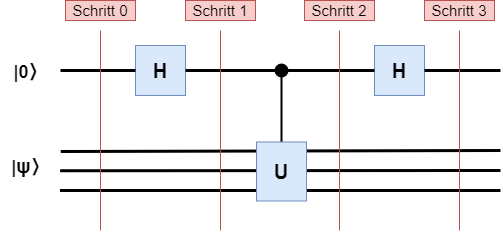
\includegraphics[width=60]{content/qpe-idea.png}
    \caption{Grundlegende Idee der Quantum Phase Estimation}
\end{figure}    \newline

Die übertragene und umgewandelte Phase von \(\Ket{\psi}\) auf das Messungsqubit kann nun gemessen werden. Dafür muss das Circuit und somit auch die anschließende Messung des Messungsqubits sehr oft wiederholt werden, und die Wahrscheinlichkeiten des Erhalts von 0 und 1 zu beobachten, wodurch sich die Phase annähernd berechnen lässt.
Durch eine genaue Betrachtung des Quantum Circuit Zustands nach jedem Schritt wird dieser Vorgang anschaulicher: \newline


\begin{align*}
     & \text{Schritt 0:}\quad \Ket{0}\Ket{\psi}                                                                                                                                                                                            \\
     & \text{Schritt 1:}\quad \frac{1}{\sqrt{2}}\begin{pmatrix}\Ket{0} + \Ket{1}\end{pmatrix}\Ket{\psi} =  \frac{1}{\sqrt{2}}\begin{pmatrix}\Ket{0}\Ket{\psi} + \Ket{1}\Ket{\psi}\end{pmatrix}                                             \\
     & \text{Schritt 2:}\quad \frac{1}{\sqrt{2}} \begin{pmatrix}\Ket{0}\Ket{\psi} + \Ket{1}\exp{(i\theta_\psi)}\Ket{\psi}\end{pmatrix}                                                                                                     \\
     & \text{Schritt 3:}\quad \frac{1}{\sqrt{2}} \begin{pmatrix}\frac{1}{\sqrt{2}}\begin{pmatrix}\Ket{0} + \Ket{1} \end{pmatrix}\Ket{\psi} + \frac{1}{\sqrt{2}}\begin{pmatrix}\Ket{0} - \Ket{1} \end{pmatrix}\exp{(i\theta_\psi)}\Ket{\psi}\end{pmatrix} \\ & \quad\quad\quad\quad\quad = \frac{1}{2} \begin{bmatrix}(1 + \exp{(i\theta_\psi)})\Ket{0} + (1 - \exp{(i\theta_\psi)})\Ket{1}\end{bmatrix}.
\end{align*}

Wie aus dem Ergebnis aus Schritt 3 die Phase geschlussfolgert werden kann, wird in einem Beispiel deutlich. Die Wahrscheinlichkeiten, die Werte 0 oder 1 zu messen, sind wie folgt:

\begin{equation}\begin{aligned}
        P(0) & = |\frac{1}{2}(1+\exp{(i\theta_\psi)})|^2  \\
        P(1) & = |\frac{1}{2}(1-\exp{(i\theta_\psi)})|^2.
    \end{aligned}\end{equation}

Wird das Circuit nun sehr oft ausgeführt und die Ergebnistabelle des Messungsqubits ergibt langfristig beispielhaft \(P(0) = 99.24\%\) und \(P(1) = 0.76\%\), so können diese angenäherten Wahrscheinlichkeiten in die Formel eingesetzt werden, um die Phase \(\theta_\psi = 10^\circ\) zu berechnen.  (Asfaw und Qiskit, Vgl. Min. 18-23) \newline
Dieser Vorgang ist ohne großen Aufwand durch die ständige Wiederholung sehr ungenau. Mit mehreren Messungsqubits kann eine höhere Genauigkeit mit weniger Wiederholungen erzielt werden. Hierfür muss das Quantum Circuit erweitert und angepasst werden.

\begin{figure}
    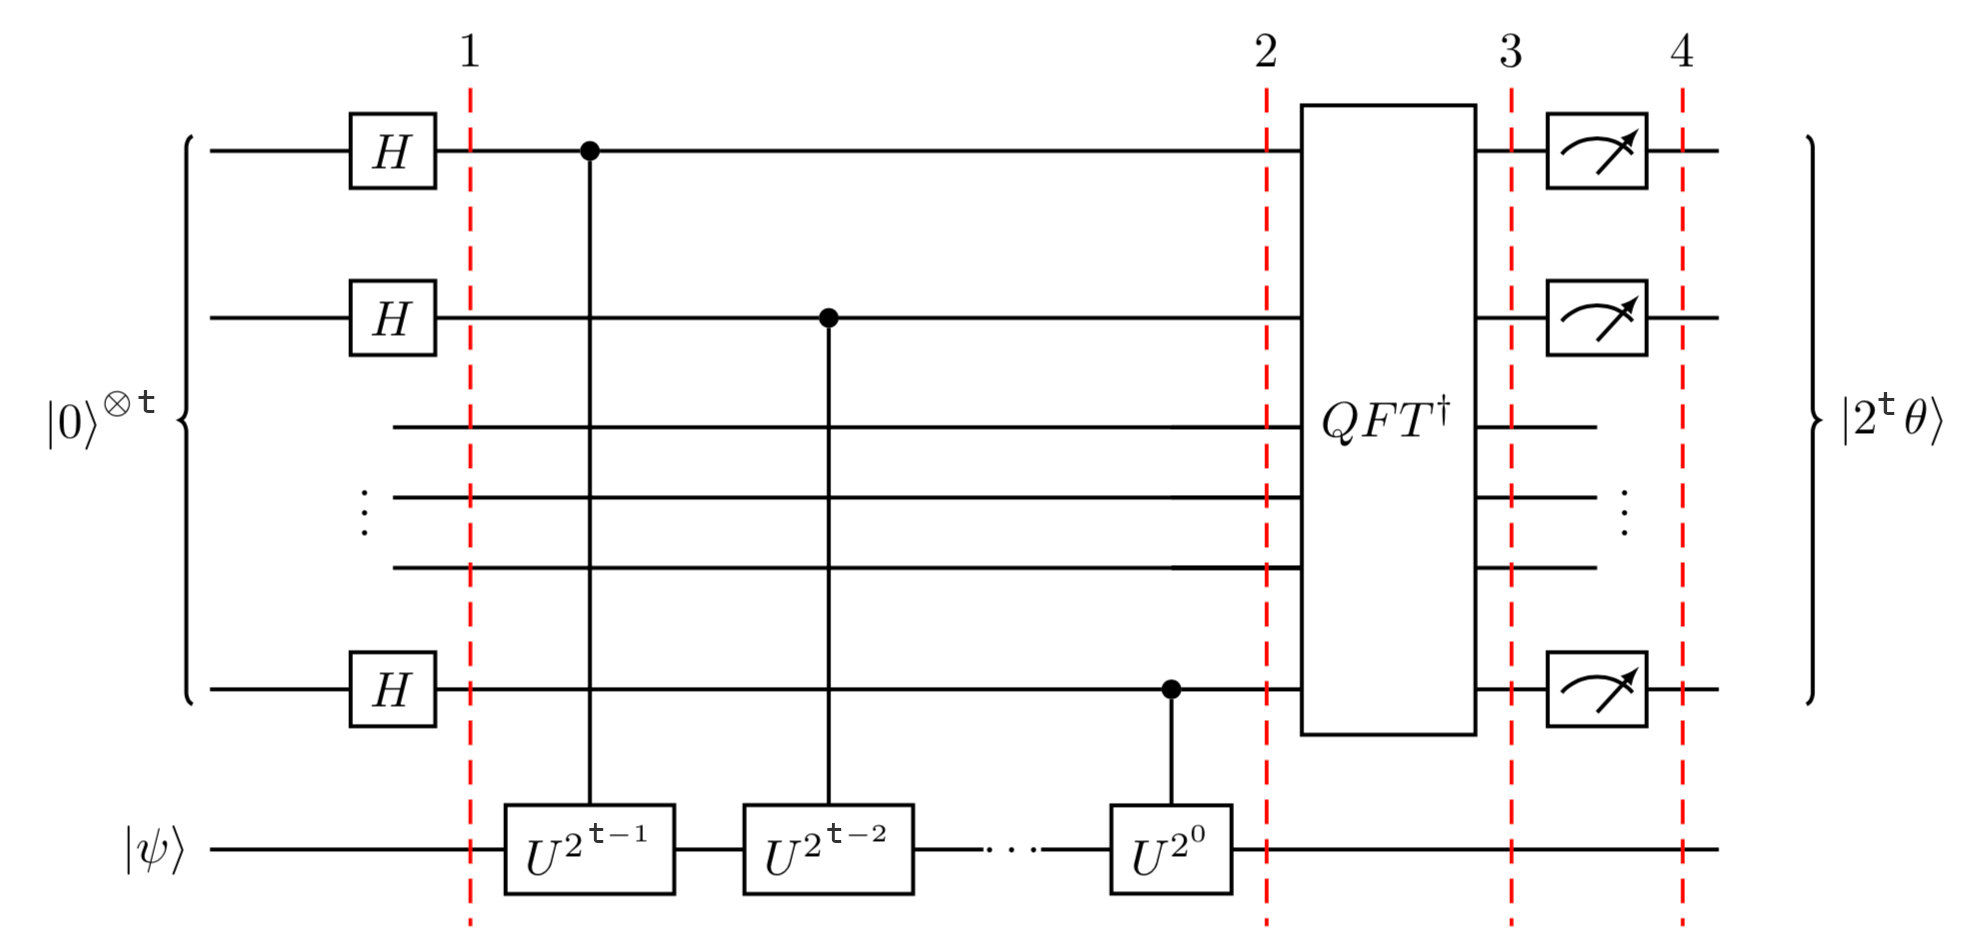
\includegraphics[width=80]{content/qpe.png}
    \caption{Quantum Phase Estimation Subroutine mit \(t\) Messungsqubits (ANIS u. a., 2021, Textbook ’Quantum Phase Estimation’ - Chapter 1)}
\end{figure}

Eine schrittweise Berechnung des Circuit Zustands verdeutlicht die Funktionsweise:

\begin{align*}
    \text{Schritt 0:}\quad & \Ket{0}^{\otimes t}\Ket{\psi}                                                                                         \\
    \text{Schritt 1:}\quad & \begin{pmatrix}
                                 \frac{1}{\sqrt{2}}\end{pmatrix}^t \begin{pmatrix}\Ket{0} + \Ket{1}\end{pmatrix}^{\otimes t}  \Ket{\psi}
\end{align*}


\hr

\textbf{Einschub:}
\(\quad U^{2^x}\Ket{\psi} = U^{2^{x-1}}U\Ket{\psi} =  U^{2^{x-1}}\exp{(i\theta_\psi)}\Ket{\psi} = U^{2^{x-2}}\exp{(i\theta_\psi)}\exp{(i\theta_\psi)}\Ket{\psi}\)
\hr


\begin{align*}
    \text{Schritt 2:}\quad & \begin{pmatrix}
                                 \frac{1}{\sqrt{2}}\end{pmatrix}^t \begin{pmatrix} \Ket{0} + \exp{(i\theta_\psi2^{t-1})}\Ket{1} \end{pmatrix} \otimes \begin{pmatrix} \Ket{0} + \exp{(i\theta_\psi2^{t-2})}\Ket{1} \end{pmatrix} ... \\
                           & \quad...\otimes \begin{pmatrix} \Ket{0} + \exp{(i\theta_\psi2^{t-t})}\Ket{1} \end{pmatrix}
    \Ket{\psi}
\end{align*}


Der Circuit Zustand nach Schritt zwei ähnelt stark dem einer QFT. \newline \newline

\hr
\textbf{Einschub:}
\(\quad QFT\Ket{x} = \Ket{\widetilde{x}} = \frac{1}{\sqrt{N}}
\begin{pmatrix}\Ket{0} + \exp{(x\cdot\frac{2\pi i}{2^1})} \Ket1\end{pmatrix} \otimes ... \otimes \begin{pmatrix}\Ket{0} + \exp{(x\cdot\frac{2\pi i}{2^n})} \Ket1\end{pmatrix}\)
\hr

\newline
\subsection{Beispiel einer QPE}
\newline

\begin{figure}
    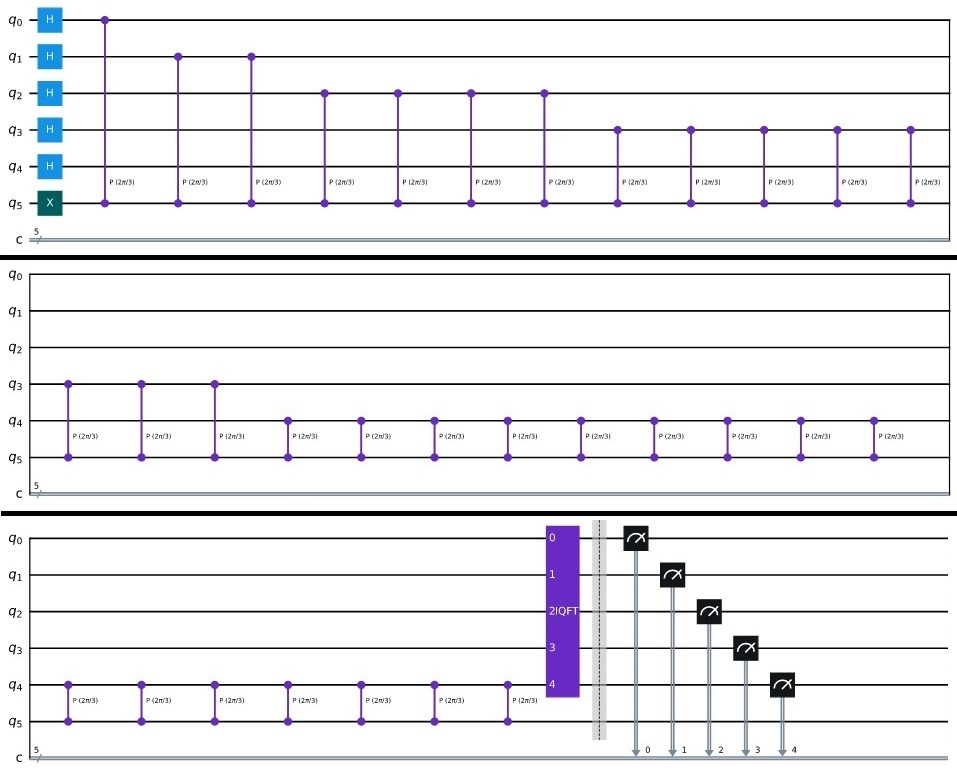
\includegraphics[width=100]{content/qpe-example.jpeg}
    \caption{Beispiel einer Quantum Phase Estimation mit unbekannter Phase \(\theta = \frac{1}{3}\) und 5 Messungsqubits  (ANIS u. a., 2021, Textbook ’Quantum Phase Estimation’ - Chapter 3)}
\end{figure}\newline

\begin{figure}
    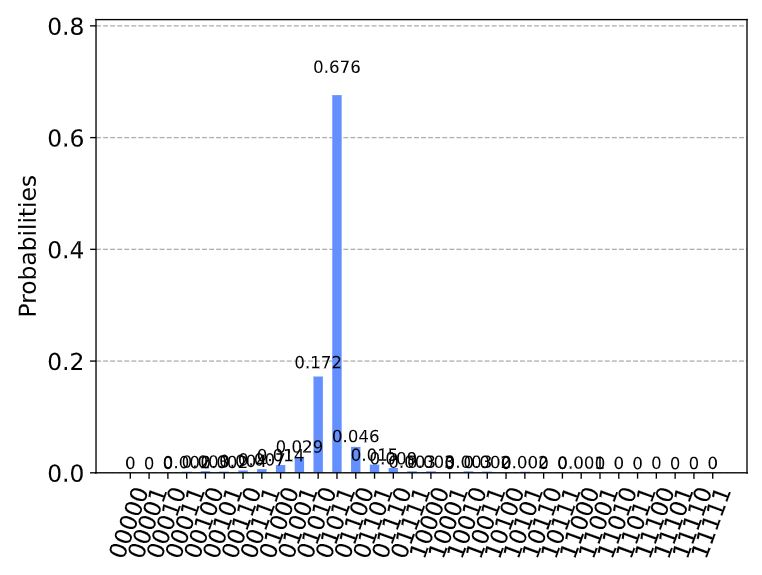
\includegraphics[width=50]{content/qpe-example-prob.JPG}
    \caption{Wahrscheinlichkeitstabelle des Beispiels in Abb. 2.12 nach 4096 Messungen  (ANIS u. a., 2021, Textbook ’Quantum Phase Estimation’ - Chapter 3)}
\end{figure}\newline

Aus der Messung des Beispiels geht hervor, dass die zwei häufigsten Ergebnisse \(01011_b = 11_{dez}\) und \(01010_b = 10_{dez}\) sind. Umgerechnet bedeutet das, dass \(\theta \approx \frac{11}{2^5} = 0.344\) oder \(\theta \approx \frac{10}{2^5} = 0.313\) ähnelt, was geringe Abweichungen von der echten Phase \(\theta = 0.334\) sind.





\newline \newline
\exercise[type=multipleChoice]{
    \question{Frage: Wieso werden so viele Messungsqubits benötigt?}
    \possibleAnswers{
        \item 1) Um mehrere Phasen zu messen.
        \item 2) Um ein genaueres Messergebnis zu erzielen.
        \item 3) Kein Qubit eines Quantencomputers darf in einer Schaltung ungenutzt bleiben.
    }
    \result{2}
}
\newline \newline
\subsection{Quellen}

[ANIS u. a. 2021] Qiskit: An Open-source Framework for Quantum Computing. 2021 \newline
[Asfaw und Qiskit ] Asfaw, Abraham ; Qiskit: Shor’s Algorithm I: Quantum Fourier Transform, Quantum Phase Estimation Part 3. – \hyperlink[url=https://www.youtube.com/watch?v=5kcoaanYyZw]{https://www.youtube.com/watch?v=5kcoaanYyZw} \newline

[Steane 2021] Steane, Andrew: Is the eigenvalue of an eigenstate the same as its (global) phase? Physics Stack Exchange. January 2021. – \hyperlink[url=https://physics.stackexchange.com/q/687904]{https://physics.stackexchange.com/q/687904} \newline